\chapter{Instalacion y Configuracion}

Este Capítulo pretende ser una guía para realizar una exitosa implementación del servidor de producción \footnote{Diferenciamos servidor de producción porque durante el desarrollo las aplicaciones en Django se prueban en un servidor virtual que crea Django para que se pueda correr la aplicación fácilmente, pero esto no es suficiente a la hora de utilizar la aplicación con usuarios finales principalmente por que el servidor de desarrollo no es lo suficientemente potente además de ser lento y consumir demasiados recursos, esta más que nada pensado para que el desarrollador pruebe la aplicación sobre él para así luego pasar a una versión de producción. } la principal consideración es que la implementación será sobre el sistema operativo Windows 7, en caso de querer instalar el sistema en otro sistema operativo, existen algunas diferencias. \\[0.5cm]

\section{Requerimientos}

\subsection{Requerimientos de Hardware}

Cualquier equipo que cumpla con las características para correr Windows 7 es suficiente en términos de requerimientos mínimos de Hardware siempre y cuando el número de usuarios esperados no sea alto, después el resto dependerá de sus necesidades. \\[0.5cm]

\begin{itemize}
    \item Procesador x86, x64 de 1.6 Ghz o superior.
    \item Memoria RAM 1 GB o Superior 
\end{itemize}


\subsection{Requerimientos de Software}


\begin{itemize}
    \item Apache 2.2
    \item PosgreSQL 9.2
    \item Python 2.7.x o Python 2.6.x
    \item Django 1.3.x o Superior
    \item PGAdmin
    \item psycopg2
    \item mod\_wsgi
    \item ReportLab
    \item easy\_thumbnails
    \item django\_extensions
    \item django\_cron
\end{itemize}


\section{Apache}

Existen 2 caminos para instalar Apache, la primera Hacer una instalación limpia de apache, la 2da es cuando no se quiere trastear con tanta configuración por lo que opta por infraestructuras tipo WAMP, LAMP, WAPP, etc. 

\subsection{Instalación en Limpio}

Solo recomiendo este tipo de instalación desde 0 para quienes ya poseen un conocimiento avanzado en cuanto al manejo de servidores. \\[0.5cm]

Descargamos de \url{Apache.org} la última versión disponible, se puede utilizar el siguiente vinculo: \url{http://www.apachehaus.com/cgi-bin/download.plx}.\\[0.5cm]

Crea dos carpetas en la unidad C, la primera de nombre {\bfseries Apache} y la segunda {\bfseries servidor}. Descomprime el archivo descargado y ejecútalo, sigue los pasos de la instalación y de los datos que te piden solo escoge el destino de la instalación, que será la carpeta que creaste en {\bfseries C:\textbackslash Apache}, los otros datos déjalos de la forma predeterminada para configurarlos más tarde. \\[0.5cm]

El programa al instalarse crea un icono en el área de notificación que te permitirá: iniciar, detener y reiniciar Apache; tienes que tener en cuenta que cualquier cambio que hagas en el archivo de configuración no tendrá efecto hasta que reinicies el servidor. \\[0.5cm]

\subsection{Instalación mediante WAMP, LAMP, MAMP, WAPP}

Existen una infinidad de Paquetes precompilados y configurados, con Apache, PHP, PosgreSQL o MySQL y más. \\[0.5cm]
Dichas infraestructuras suelen nombrarse como el acronomico de las herramientas que agrupan por ejemplo:\\[0.5cm]

\begin{itemize}
    \item {\large WAMP {\bfseries W}indows {\bfseries A}pache {\bfseries M}ySQL {\bfseries P}HP}
    \item {\large WAPP  {\bfseries W}indows {\bfseries A}pache {\bfseries P}osgreSQL {\bfseries P}HP}  
    \item {\large LAMP {\bfseries L}inux {\bfseries A}pache {\bfseries M}ySQL {\bfseries P}HP} 
    \item {\large MAMP {\bfseries M}ac OS {\bfseries A}pache {\bfseries M}ySQL {\bfseries P}HP}  
\end{itemize}


Algunas de las distribuciones más usadas disponibles Para Windows son :\\[0.5cm]
\begin{itemize}
    \item WAMP Server \url{http://www.wampserver.com/} (WAMP),
    \item XAMPP \url{http://sourceforge.net/projects/xampp/} 
    \item (WAMP + Perl), Bitnami \url{http://bitnami.com/stack/wapp} (WAPP)
\end{itemize}

Solo nos resta elegir cualquiera de ellas e instalarlas, aparte de la ruta de instalación nos pedirán el usuario y
contraseña para acceder al motor de Base de Datos.

\subsection{Configuración}

Toda la configuración para el funcionamiento de Apache se guarda en un archivo de texto nombrado: {\bfseries httpd.conf} que se encuentra en la ruta {\bfseries C:\textbackslash Apache \textbackslash conf } si realizamos una instalación en limpio o {\bfseries C:\textbackslash WAMP \textbackslash bin \textbackslash  Apache \textbackslash conf } si instalamos el paquete múltiple preconfigurado no es necesario realizar este paso por lo que lo podremos saltar. \\[0.5cm]


Al archivo {\bfseries httpd.conf} lo podemos editar en cualquier editor de texto como Notepad o algo más avanzado como Notepad++, Geany, etc. \\[0.5cm]

Buscamos la línea que dice

\begin{lstlisting}[style=consola, numbers=none]
    Listem LocalHost:80
\end{lstlisting}

Y la Cambiamos por:

\begin{lstlisting}[style=consola, numbers=none]
    Listem 80
\end{lstlisting}

Ahora buscamos la instrucción:

\begin{lstlisting}[style=consola, numbers=none]
    DocumentRoot "C:\xxxxxxxx"
\end{lstlisting}

La Cambiamos por:

\begin{lstlisting}[style=consola, numbers=none]
    DocumentRoot "C:\Servidor"
\end{lstlisting}

Recordar que al inicio de la instalación creamos una carpeta llamada Servidor en la unidad C. Por último solo nos queda reiniciar el servidor Apache e introducir la siguiente dirección \url{http://127.0.0.1} si nos aparece una página {\bfseries It's Work!} felicidades Apache está Funcionando. El problema más común por lo que aveses apache no inicia se debe a que el puerto puede estar siendo utilizado por otra aplicación como Skype, para ello asegúrese antes de que el puerto 80 este libre o utilice otro puerto como el 8080.


\subsection{Instalación de PosgreSQL}

La versión de PostgreSQL que he utilizado durante el desarrollo del sistema es la 9.2.x, quizás cuando leas esto ya halla salido una nueva versión la cual no debería generar inconvenientes además de que es posible que el proceso de instalación pueda variar.\\[0.2cm]
 
El primer paso es descargar el instalador de PostgreSQL para Windows, el cual puedes descargar desde el enlace siguiente \url{http://www.postgresql.org/download/windows}, nos bajara un instalador similar
a {\bfseries postgresql-9.2.3-rc1-windows.exe} lo ejecutamos como administrador.\\[0.2cm]

Si tenemos activado el control de cuentas de usuario nos mostrara una advertencia con el texto "¿Desea permitir que este programa realice cambios en el equipo?", pulsaremos "Sí" para continuar con la instalación de PostgreSQL.\\[0.2cm]

Indicaremos la carpeta de instalacion de PostgreSQL, donde se guardarán los ejecutables, librerías y ficheros de configuración de PostgreSQL en mi caso el directorio es {\bfseries C: \textbackslash PostgreSQL \textbackslash 9.2 }, Indicaremos también la carpeta donde se guardarán los datos por defecto de PostgreSQL {\bfseries C: \textbackslash psql-data }.\\[0.2cm]

Solo nos queda introducir la contraseña para el súper usuario "postgres" \footnote{Puedes cambiar la contraseña y crear un nuevo usuario para aumentar la seguridad del sistema solo recuerda que deberás cambiar la configuración de Django para que este pueda conectarse a la base de datos con un usuario diferente.} que será con el que iniciemos sesión para administrar la base de datos, después podremos crear otros usuarios si es necesario. Además introduciremos el puerto de escucha para la conexión con el servidor PostgreSQL, por defecto el 5432.\\[0.2cm]

Seleccionaremos la configuración regional y comenzara la instalación, con esto PostgreSQL quedara instalado. Si tenemos algún cortafuego (firewall) deberemos abrir el puerto 5432.

\subsection{Creación de la Base de Datos}

Junto con la Instalación de PosgreSQL se instala el PGAdmin III que es una herramienta GUI\footnote{GUI (del inglés \textit{graphical user interface}) es un programa informático que actúa de interfaz de usuario, utilizando un conjunto de imágenes y objetos gráficos para representar la información y acciones disponibles en la interfaz} para administrar el motor de base de Datos. Iniciamos el Programa, desplegaremos "Server Groups", dentro desplegaremos "Servidores" y dentro de éste pulsaremos con el botón derecho del ratón sobre "PostgreSQL 9.0 (localhost:5432), en el menú emergente seleccionaremos "Conectar".

Introduciremos la contraseña para el súper usuario postgres (la contraseña introducida en la instalación).

Pulsaremos con el botón derecho del ratón sobre "Bases de datos", seleccionaremos "Nueva Base de Datos", en la pestaña "Propiedades" introduciremos los siguientes datos:

\begin{itemize}
    \item Nombre: nombre de la base de datos, en nuestro caso "BDSem".
    \item Propietario: seleccionaremos el usuario creado anteriormente "posgres".
    \item Codificado: seleccionaremos UTF8.
    \item Tablespace: seleccionaremos el tablespace creado anteriormente "pg\_default".
    \item Colación: seleccionaremos "Spanish, Argentina".
    \item Tipo carácter: seleccionaremos "Spanish, Argentina".
\end{itemize}

Pulsaremos OK para crear la base de datos, con esto ya tendremos nuestra base de datos aunque vacía, el resto como creación de las Tablas correspondientes necesarias para el proyecto lo haremos más adelante mediante Django.



\section{Instalación de Python}

Para este proyecto se utilizo CPython pero no la versión Oficial url{http://www.python.org} sino la que distribuye Active State \url{http://www.activestate.com} llamada {\bfseries Active Python} la cual provee características adicionales a versión oficial, podremos descargar la ultima versión desde  \url{http://www.activestate.com/activepython/downloads} aunque se recomienda instalar la version 2.7.x para evitar cualquier posible problema ya que es incompatible con las versión 3.x de Python.

\subsection{Probando Python}
Para probar que la instalación haya sido correcta abriremos la Terminal \textbf{cmd.exe} y escribiremos:

\begin{lstlisting}[style=consola, numbers=none]
    python
\end{lstlisting} 

Si todo va bien nos deberá aparecer algo similar a:

\begin{figure}[h]
    \centering
    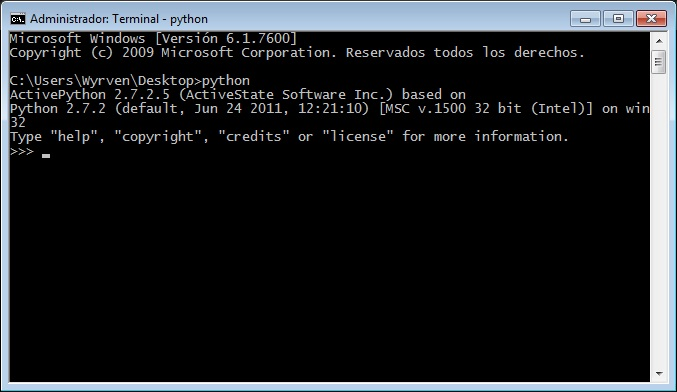
\includegraphics[scale=0.7]{resourse/consola-python.jpg}
    \caption{Ejecutando Python en la Terminal}
    \label{fig:01}
\end{figure}    

En caso contrario deberías revisar que la ruta de Python este dentro de la variable  PATH del sistema.


\section{Instalar Django}

Puedes bajarte Django desde el siguiente enlace \url{https://www.djangoproject.com/download/1.3.7/tarball/}
\footnote {la versión 1.3.7 no es la última versión disponible a la hora de crear este informe estaba por la 1.6.2 ya que Django se actualiza constantemente.} te descargara un paquete llamado Django-1.3.7.tar.gz lo descomprimes en algún directorio luego abres la Terminal y te posicionas sobre el directorio donde descomprimiste y ejecutas:

\begin{lstlisting}[style=consola]
    $ python setup.py install 
\end{lstlisting}
\vspace{0.1cm}

Sino mediante el instalador de Paquetes de Python de manera más automática escribes en la terminal

\begin{lstlisting}[style=consola]
     pip install django==1.3.7
\end{lstlisting}
\vspace{0.1cm}

Con esto ya tendremos instalado Django.

\section{Instalando el Resto de Las Dependencias}

Ademas de Django en el proyecto se utilizaron otras librerías de Python las cuales algunas vienen instaladas y otras requieren ser instaladas de manera similar a como instalamos Django.

\subsection{psycopg2}

psycopg2 es un adaptador de base de datos PostgreSQL para el lenguaje de programación Python. psycopg2 fue escrito con el objetivo de ser muy pequeño y rápido y estable. 

psycopg2 es diferente del otro adaptador de base de datos, ya que fue diseñado para aplicaciones en gran medida de subprocesos múltiples que crean y destruyen un montón de cursores y hacen que un número notable de inserciones o actualizaciones concurrentes. psycopg2 también proporcionan operaciones asincrónicas completas y apoyo a las bibliotecas de co-rutinas. 

Para instalar descargue el precompilado desde \url{http://www.stickpeople.com/projects/python/win-psycopg/} ejecútelo con permisos de administrador, nos pedirá que seleccionemos la versión de Python con que se instalar. \footnote{Se podría instalar usando el código fuente con pip pero para ello se requiere tener alguna versión del compilador Visual C++ ya que parte de la librería fue portada desde C++}

\subsection{ReportLab}

ReportLab es la ultra-robusto motor de código abierto a prueba de tiempo para la creación de documentos PDF y gráficos vectoriales personalizado. Escrito en Python, ReportLab es rápido, flexible y una plataforma cruzada (funciona tanto en Linux como Windows).
 
Proporciona un completo conjunto de herramientas de programación para la creación de documentos y gráficos complejos. Ofrecemos una serie de componentes de forma gratuita y de código abierto, además de un paquete comercial con características adicionales.

Para Instalar descargue el instalado desde \url{http://www.reportlab.com/software/installation/} y proceda de manera similar a como hizo con la instalacion de psycopg2.


\subsection{easy\_thumbnails}

Easy\_Thumbnails es una potente aplicación thumbnailing \footnote{Cuando hablamos de thumbnails nos referimos a las diferentes miniaturas que son versiones en distintos tamaños  de una imagen y son usadas para ayudar a su organización y reconocimiento.}, pero fácil de implementación para Django.

Para Instalar solo ejecute el siguiente comando en terminal, no se necesita configurar nada en el proyecto el mismo esta previamente configurado.

\begin{lstlisting}[style=consola]
    pip install easy-thumbnails
\end{lstlisting}
\vspace{0.1cm}

\subsection{django\_extensions}

Django\_Extensions es una colección de Extensiones (utilidades) Personalizadas de diferentes autores no relacionados con el Proyecto Django, para extender las capacidades del Framework.

Para Instalar solo ejecute el siguiente comando en terminal \footnote{Importante, no todas las funcionalidades están soportadas en Windows, pero en cuanto a la requeridas por el proyecto no hay problemas.}

\begin{lstlisting}[style=consola]
     pip install django-extensions
\end{lstlisting}
\vspace{0.1cm}


\subsection{django\_cron}

Django-cron permite ejecutar código de Django de manera recurrente para el seguimiento y ejecución de las tareas. En este caso no es necesario Instalar nada, se adjunto con el código fuente del Proyecto. Igualmente si tiene curiosidad puede visitar la página del proyecto \url{https://github.com/Tivix/django-cron}

\subsection{Descargar e Instalación de mod\_wsgi}

 Asumiendo que ya  tienes instalado Python y Apache, solo debes descargar el paquete  libapache2-mod-wsgi ,la ultima versión de mod\_wsgi se puede descargar desde su  página oficial  \url{https://code.google.com/p/modwsgi/} descargaran un archivo  similar a "mod\_wsgi-win32-ap22py27-3.3.so" la versión que descarguen de mod\_wsgi  depende como se ve, de la plataforma así como de la versión de Python que  correrá en el servidor, luego por cuestiones de practicidad renombraremos  el archivo de la siguiente manera:

\begin{lstlisting}[style=consola]
    mod_wsgi-win32-ap22py27-3.3.so -> mod_wsgi.so
\end{lstlisting}
\vspace{0.1cm}

Realizado dicho cambio copiamos el modulo dentro de la siguiente carpeta: APACHE\_FOLDER \textbackslash modules \textbackslash APACHE\_FOLDER vendría a ser el directorio donde tenemos la instalación de WAMP en mi caso es: 

C:\textbackslash Apache.

\subsection{Cargando el Modulo en Apache}

Una vez que el módulo de Apache ha sido instalado en el directorio de módulos de su instalación de Apache, todavía es necesario configurar Apache para cargar el módulo en realidad.

Abrimos el archivo \textbf{httpd.conf} y agregamos la siguiente línea en el mismo punto donde se cargan el resto de los módulos. \footnote {El archivo httpd.conf esta en la siguiente ruta en el caso de mi instalación: C:\textbackslash Apache \textbackslash conf \textbackslash httpd.conf}

\begin{lstlisting}[style=consola]
    LoadModule wsgi_module modules/mod_wsgi.so
\end{lstlisting}
\vspace{0.1cm}

Con todo esto hecho solo tenemos que reiniciar el servidor Apache, en nuestro  caso clic en el icono en la barra de notificaciones luego las opciones  Apache->Service->Reiniciar Servicio. 

\section{Configuracion del Proyecto}

Bueno Ahora solo tenemos que crear un alias en Apache \footnote{Para mayor información de cómo crear alias en Apache consulte \url{http://httpd.apache.org/docs/2.2/urlmapping.html}} para nuestra carpeta donde colocaremos en mi caso la carpeta destino será:

\begin{lstlisting}[style=consola]
	C:\Servidor\SGCM
\end{lstlisting}
\vspace{0.1cm}

SGCM es la carpeta contenedora del proyecto, y el alias que usaremos será:

\begin{lstlisting}[style=consola]
	/sgcm/ 
\end{lstlisting}
\vspace{0.1cm}

Tendremos que agregar las siguientes líneas al final del archivo httpd.conf de apache.

\begin{lstlisting}[style=HTML]
Alias /sgcm/ "C:/Servidor/SGCM/" 
WSGIScriptAlias /sgcm "C:/Servidor/SGCM/handle.wsgi" 

<Directory "C:/Servidor/SGCM">
    Options Indexes FollowSymLinks MultiViews
    AllowOverride all
    Order allow,deny
    Allow from all
</Directory>
\end{lstlisting}
\vspace{0.1cm}


Hay un número de maneras en que puede instalar una aplicación WSGI organizada por mod\_wsgi
Puede consultar \url{https://code.google.com/p/modwsgi/wiki/QuickInstallationGuide} si desea explorar otras opciones de configuración.

Puede montarse contra una URL específica. Estos métodos son similares a cómo se podría configurar las aplicaciones CGI tradicionales.

El principal enfoque implica declarar explícitamente en el archivo de configuración principal de Apache el punto de montaje URL y una referencia al archivo de comandos de aplicaciones WSGI. En este caso, el mapeo se fija, con cambios sólo ser capaz de ser hecho mediante la modificación de la configuración principal de Apache y reiniciar Apache.

Al utilizar mod\_cgi para alojar aplicaciones CGI, esto se haría mediante la directiva ScriptAlias. Para mod\_wsgi, la directiva en su lugar se llama WSGIScriptAlias.

\begin{lstlisting}[style=consola]
WSGIScriptAlias /wsgi "C:/Servidor/SGCM/handle.wsgi" 
\end{lstlisting}
\vspace{0.1cm}

Esta directiva solo puede aparecer en los principales archivos de configuración de Apache. La directiva se puede utilizar en el ámbito del servidor, pero normalmente se coloca en el contenedor VirtualHost para un sitio en particular. No se puede utilizar en cualquiera de las directivas de contenedores ubicación, directorios o archivos, ni puede ser utilizada dentro de un archivo ''.httaccess''.

El primer argumento de la directiva WSGIScriptAlias debe ser el punto de montaje URL para la aplicación WSGI. En este caso, la URL no debe contener una barra diagonal. La única excepción a esto es si la aplicación WSGI es para ser montado en la raíz del servidor web, en cuyo caso / sería utilizado.

El segundo argumento de la directiva WSGIScriptAlias debe ser una ruta absoluta para el archivo de comandos de aplicaciones WSGI. Es en este archivo que la muestra de código de la aplicación WSGI debe colocarse.

Tenga en cuenta que una ruta absoluta debe ser utilizado para el archivo de comandos de aplicaciones WSGI suministrado como segundo argumento. No es posible especificar una aplicación por si  sola Python nombre de módulo. Una ruta de acceso completa se utiliza para una serie de razones, la principal de las cuales por lo que todos los controles de acceso de Apache todavía pueden aplicarse para indicar que en realidad puede acceder a la aplicación WSGI.

Porque se aplicarán los controles de acceso de Apache, si la aplicación WSGI se  encuentra fuera de los directorios que ya están configurados para ser accesible a Apache, habrá que decirle a Apache que los archivos dentro de ese directorio se   pueden utilizar. Para ello se debe utilizar la directiva Directory.

Hasta aqui tenemos mod\_wsgi y nuestro directorio listo, ahora probaremos que todo va bien para ello dentro del directorio crearemos un archivo llamado "handle.wsgi" que tendra el siguiente contenido:

\begin{lstlisting}[style=Python]
# -*- coding: utf-8 -*-

import os, sys
import django.core.handlers.wsgi

sys.path.append('C:/Servidor/SGCM')
sys.path.append('C:/Servidor')

os.environ['DJANGO_SETTINGS_MODULE'] = 'settings'

application = django.core.handlers.wsgi.WSGIHandler()

\end{lstlisting}
\vspace{0.1cm}


Con esto nuestro servidor de aplicación ya debería funcionar aunque como verán no se cargan los archivos estáticos como imágenes y hojas de estilo por lo que necesitamos agregarlo.

Django no debería ser utilizado para servir archivos multimedia (imagen, audio, video, flash) por sí mismo; mejor deja ese trabajo al servidor web que hayas elegido. Recomendamos usar un servidor Web separado (es decir, uno que no está corriendo a la vez Django) para servir estos archivos. 

Sin embargo, si no tienes opción para servir los archivos multimedia que no sea el mismo VirtualHost Apache que usa Django, aquí te mostramos como desactivar mod\_python para una parte particular del sitio agregando la siguiente información a http.conf:

\begin{lstlisting}[style=consola]
<Location "/media/">
    SetHandler None
</Location>
\end{lstlisting}
\vspace{0.1cm}

Cambia \textbf{Location} a la URL raiz donde se encuentran tus archivos.

También puedes usar \textit{<LocationMatch>} para comparar con una expresión regular. Por ejemplo, esto configura Django en la raíz del sitio pero deshabilitando Django para el subdirectorio media y cualquier URL que termine en .jpg, .gif, o .png:

\begin{lstlisting}[style=consola]
<Location "/">
    SetHandler python-program
    PythonHandler django.core.handlers.modpython
    SetEnv DJANGO_SETTINGS_MODULE mysite.settings
</Location>

<Location "/media/">
    SetHandler None
</Location>

<LocationMatch "\.(jpg|gif|png)$">
    SetHandler None
</LocationMatch>
\end{lstlisting}
\vspace{0.1cm}

En todos estos casos, necesitarás configurar la directiva \textbf{DocumentRoot} para que Apache sepa dónde encontrar tus archivos estáticos.

Con esto Django estará funcionando correctamente, y podrá cargar imágenes y demás ficheros necesarios.


\section{Configuración Inicial}

Ahora que tenemos todo instalado y funcionando, debemos crear la configuración inicial necesaria para que la aplicación pueda funcionar ya que si intentamos acceder en este momento a la aplicación nos devolverá una serie de errores, por faltar información, entre ellas que todavía no se crearon las tablas necesarias para soportar el modelo y los datos de los mismos.

Empecemos creando las tablas necesarias, se supone que la base de datos ya esta creada y su nombre agregado en el archivo \textbf{setings.py} ósea suponemos que hicimos todos los pasos necesarios para conectar la base de datos y demás bueno en la ruta donde localizamos el proyecto ejecutamos el siguiente comando desde terminal:

\begin{lstlisting}[style=consola]
$ python manage.py syncdb
\end{lstlisting}

Esta instrucción le dice a Django que sincronice los modelos con la base de datos y que cree las tablas necesarias en la misma para que esto funcione, además no preguntara si deseamos crear una cuenta para el administrador debemos decir si, y proporcionar el nombre de la misma, el cual por requerimiento el nombre del usuario administrador debe ser \textbf{admin}, este requerimiento es necesario para luego lanzar e implementar la configuración inicial.

Con las tablas creadas y el usuario admin creados, procedemos a crear la información necesaria para el funcionamiento de la aplicación, para ello ejecutaremos el siguiente script:

\begin{lstlisting}[style=consola]
$ python init_app.py
\end{lstlisting}

El mismo creara toda la información requerida por la aplicación y con ello quedara nuestro servidor en funcionamiento, solo hará falta reiniciar Apache. Con esto concluye todo lo referente a configuración del servidor.







%%%




